\documentclass[a4paper,12pt,oneside]{report}
\usepackage{array}
\usepackage{enumitem}
\usepackage[utf8]{inputenc}
\usepackage{emptypage}
\usepackage{graphicx}
\usepackage[table]{xcolor}
\usepackage{glossaries}
\usepackage{dirtytalk}
\renewcommand{\baselinestretch}{1.5}
\usepackage{geometry}
\geometry{
 a4paper,
 total={170mm,257mm},
 left=1.2in,
 top=1in,
 bottom=1.25in,
 right=1in
}
\usepackage{sectsty}
\usepackage{fancyhdr}
\usepackage{tocloft}
\usepackage{tabularx}
\usepackage{booktabs}
\usepackage{longtable}
\usepackage{float}
\usepackage{tikz}
\usepackage{pgfplots}
\pgfplotsset{compat=1.18}
\usepackage[hidelinks]{hyperref}
\setlength{\emergencystretch}{3em}

\chapternumberfont{\vspace{-2 cm} \centering \Large \MakeUppercase}
\chaptertitlefont{\vspace{-0.5 cm} \centering \Large \MakeUppercase}
\sectionfont{\large\uppercase}
\subsectionfont{\large}

\newcommand{\changefont}{%
\fontsize{10}{12}\selectfont
}
\newcommand{\listequationsname}{List of Equations}
\newlistof{myequations}{equ}{\listequationsname}
\newcommand{\myequations}[1]{%
\addcontentsline{equ}{myequations}{\protect\numberline{\theequation}#1}\par}
\renewcommand{\contentsname}{CONTENTS}
\renewcommand{\listfigurename}{LIST OF FIGURES}
\renewcommand{\cfttoctitlefont}{\hspace*{\fill}\large\bfseries}
\renewcommand{\cftaftertoctitle}{\hspace*{\fill}}
\renewcommand{\cftlottitlefont}{\hspace*{\fill}\large\bfseries}
\renewcommand{\cftafterlottitle}{\hspace*{\fill}}
\renewcommand{\cftloftitlefont}{\hspace*{\fill}\large\bfseries}
\renewcommand{\cftafterloftitle}{\hspace*{\fill}}

\newcommand{\ProjectTitle}{ISOLENS: INTELLIGENT DYNAMIC MALWARE ANALYSIS SANDBOX}
\newcommand{\Placeholder}[1]{\textbf{[INSERT #1]}}
\newcommand{\ScreenshotPlaceholder}[2]{
\begin{figure}[H]
\centering
\fbox{\parbox[c][#2][c]{0.88\textwidth}{\centering \textbf{Screenshot Placeholder}\\[4pt] #1}}
\caption{#1}
\end{figure}
}
\newcommand{\DiagramPlaceholder}[2]{
\begin{figure}[H]
\centering
\fbox{\parbox[c][#2][c]{0.88\textwidth}{\centering \textbf{Diagram Placeholder}\\[4pt] #1}}
\caption{#1}
\end{figure}
}

\begin{document}

\begin{titlepage}
\addtolength{\hoffset}{0cm}
\centering
{\scshape\large \bfseries \ProjectTitle\par}
\vspace{0.6cm}
{\scshape \bfseries A PROJECT REPORT \par}
\vspace{0.3cm}
{\small \bfseries submitted by \par}
\vspace{0.3cm}
\begin{center}
\large\bfseries
\begin{tabular}{@{}l l@{}}
ATHUL PRAKASH N J & MUT23CC022 \\
\end{tabular}
\end{center}
\vspace{0.3cm}
{\small \bfseries to \par}
\vspace{0.3cm}
{\small \bfseries the APJ Abdul Kalam Technological University in partial fullfilment of the requirements for the award of the Degree \par}
\vspace{0.3cm}
{\small \bfseries of \par}
\vspace{0.3cm}
{\bfseries Bachelor of Technology\par}
{ In \par}
{\bfseries Computer Science \& Engineering (Cyber Security)\par}
\vspace{0.3cm}

\includegraphics[width=0.42\textwidth]{figure/Master Logo-transparent 1.png}\par\vspace{0.7cm}
{\bfseries Department of Cyber Security\par}
{\bfseries Muthoot Institute of Technology and Science\par}
{\bfseries Varikoli PO, Puthencruz - 682308 \par}
\vspace{0.7cm}
{\bfseries MARCH 2026 \par}
\end{titlepage}

\begin{titlepage}
{\scshape \centering \Large \bfseries DECLARATION \par}
\vspace{1.5cm}
{I hereby declare that this submission is my own work and that, to the best of my knowledge and belief, it contains no material previously written by another person nor material which has been accepted for the award of any other degree or diploma of the university or other institute of higher learning, except where due acknowledgment has been made in the text.}
\vspace{2cm}
\begin{flushright}
\begin{tabular}{lr}
\textbf{ATHUL PRAKASH N J} & \textbf{MUT23CC022} \\
\end{tabular}
\end{flushright}
\par

\vfill
\noindent Place: ERNAKULAM\\
\noindent Date: 26-03-2026
\end{titlepage}

\begin{titlepage}
\vspace{1.5cm}
\begin{center}

\includegraphics[width=0.50\textwidth]{figure/Master Logo-transparent 1.png}\par\vspace{1cm}
{\scshape \Large \bfseries CERTIFICATE \par}
\end{center}
\par

\noindent
\textit{This is to certify that the report entitled} \textbf{``\ProjectTitle''}, \textit{submitted by} \textbf{ATHUL PRAKASH N J} \textit{to Muthoot Institute of Technology and Science, Varikoli for the award of the degree of Bachelor of Technology in Computer Science \& Engineering (Cyber Security) is a bonafide record of the project work carried out under our supervision and guidance. The content of the report, in full or parts, has not been submitted to any other Institute or University for the award of any other degree or diploma.}
\vspace{2.5cm}
\par\noindent
\begin{center}
\renewcommand{\arraystretch}{1.2}
\setlength{\tabcolsep}{0pt}
\begin{tabular*}{\textwidth}{@{\extracolsep{\fill}}ccc}
\textbf{SAFAD ISMAIL} & \begin{tabular}[t]{@{}c@{}}\textbf{Ms. SREEJA S,}\\ \textbf{Ms. SNEHA THANKACHAN}\end{tabular} & \textbf{Dr VICKY NAIR} \\[0.2cm]
Asst. Professor & Asst. Professor(s) & Head of the Department \\
Dept. of Cyber Security & Dept. of Cyber Security & Dept. of Cyber Security \\
Project Guide & Project Coordinators & \\
\end{tabular*}
\end{center}

\vfill
\noindent Place: ERNAKULAM\\
\noindent Date: 26-03-2026
\end{titlepage}

\newpage
\pagenumbering{roman}
\setcounter{page}{1}
\thispagestyle{plain}
\begin{center}
\section*{ACKNOWLEDGMENT}
\end{center}
\addcontentsline{toc}{section}{ACKNOWLEDGMENT}

\noindent
I express my sincere gratitude to all those who supported the successful completion of this mini project. I thank my project guide \textbf{SAFAD ISMAIL}, the project coordinators \textbf{Ms. SREEJA S and Ms. SNEHA THANKACHAN}, and \textbf{Dr. VICKY NAIR}, Head of the Department of Cyber Security, for their guidance, technical inputs, and consistent encouragement throughout the work.

\par

\par

I are grateful to the faculty and staff of Muthoot Institute of Technology and Science for providing the academic environment and infrastructure needed to complete this project. I also thank my institution for enabling me to work on a practical cybersecurity problem with direct relevance to malware analysis and secure systems engineering.

\par

\par

Finally, I acknowledge the support of my peers and well-wishers who contributed suggestions, testing assistance, and feedback during the design and implementation of IsoLens.

\newpage
\pagenumbering{roman}
\setcounter{page}{2}
\thispagestyle{plain}
\begin{center}
\section*{ABSTRACT}
\end{center}
\addcontentsline{toc}{section}{ABSTRACT}
\par

IsoLens~\cite{isolens} functions as an academic malware sandbox prototype that is designed to execute suspicious files inside an isolated Windows virtual machine and automatically generate a structured behavioral analysis report. The system combines virtualization, host-side orchestration, guest-side artifact collection, web-based interaction, and AI-assisted threat interpretation into a single modular platform. The implemented workflow allows a user to upload a suspicious file through a browser interface, transfer the file into a sandbox environment, execute it in a controlled setting, collect behavioral artifacts such as process activity, network activity, file and registry traces, and screenshots, and finally consolidate these findings into a readable threat assessment.

\par

\par

My architecture is separated into distinct layers for the user interface, API gateway, orchestration controller, guest agent, collector modules, storage, and threat intelligence processing. VirtualBox is used to isolate the guest environment, while the in-VM agent manages execution and artifact packaging. The final implementation also includes an AI analysis layer that processes collected artifacts and produces summaries, threat classification, indicators of compromise, recommendations, and MITRE ATT\&CK mappings.

\par

\par

IsoLens is intentionally lightweight and academic in scope. It prioritizes modularity, explainability, and practical demonstration over production-scale complexity. The project shows how automated dynamic analysis and AI-based summarization can be combined to improve malware triage in a secure and educational environment.

\newpage
\tableofcontents

\newpage
\listoffigures
\addcontentsline{toc}{section}{LIST OF FIGURES}

\newpage
\listoftables
\addcontentsline{toc}{section}{LIST OF TABLES}

\newpage
\chapter*{\uppercase{List of Abbreviations}}
\addcontentsline{toc}{section}{LIST OF ABBREVIATIONS}
\begin{table}[H]
\renewcommand{\arraystretch}{1.5}
\begin{tabularx}{\textwidth}{>{\bfseries}l X}
API & Application Programming Interface \\
DFD & Data Flow Diagram \\
GUI & Graphical User Interface \\
IOC & Indicator of Compromise \\
LLM & Large Language Model \\
VM & Virtual Machine \\
OS & Operating System \\
\end{tabularx}
\end{table}

\newpage


\newpage
\renewcommand\thepage{\arabic{page}}
\clearpage
\setlength{\headheight}{15pt}
\pagestyle{fancy}
\fancyhf{}
\lhead{\changefont\thechapter.\leftmark}
\rhead{}
\cfoot{\thepage}
\renewcommand{\chaptermark}[1]{\markboth{#1}{}}
\renewcommand{\sectionmark}[1]{\markright{#1}{}}
\renewcommand{\headrulewidth}{0.5pt}
\pagenumbering{arabic}
\setcounter{page}{1}

\chapter{INTRODUCTION}
\noindent
Analyzing malware safely is a highly critical activity in cybersecurity because suspicious executables often need to be examined before they are trusted inside a real environment. Static analysis can reveal signatures, embedded strings, and binary metadata, but many modern threats use packing, delayed execution, sandbox detection, or staged behavior that become visible only during runtime. For this reason, dynamic analysis inside an isolated environment remains one of the most effective methods for understanding the behavior of unknown software.

\par

\par

I developed IsoLens as a lightweight mini-project to demonstrate an end-to-end malware sandbox workflow using accessible tools and a modular software architecture. The system executes suspicious samples inside a Windows virtual machine, collects multiple categories of runtime artifacts, stores the resulting evidence in a structured report directory, and augments the final report using AI-assisted threat intelligence. The project is positioned as an educational prototype rather than a production-grade commercial sandbox.

\section{Motivation}
\noindent
My motivation for this project stems from the need for an affordable and understandable malware analysis pipeline for academic use. Commercial sandboxes offer rich functionality but are expensive, closed, and difficult to study internally. At the same time, a purely conceptual academic report would not sufficiently demonstrate implementation depth. IsoLens addresses this gap by building a working system that includes user interaction, execution isolation, behavioral monitoring, and automated report generation.

\par

\par

The scope of the current project is intentionally bounded. IsoLens focuses on Windows-based sample execution in an isolated virtual machine, sequential analysis of one sample at a time, file-based storage of generated reports, and AI-generated interpretation of collected evidence. Features such as multi-user authentication, distributed workers, memory forensics, and multi-platform sandboxing are treated as future extensions rather than part of the current implementation.

\section{Problem Statement}
Security researchers frequently encounter suspicious files that cannot be trusted for direct execution on a host machine. Manual analysis is slow, requires specialized expertise, and does not scale well. Static inspection alone often misses behavior that appears only at runtime. Therefore, there is a need for a controlled and automated system that can execute suspicious files in isolation, observe their behavior, collect relevant evidence, and transform the collected data into an understandable report for security analysts and students.

\chapter{LITERATURE REVIEW}
\section{Improving the Efficiency of Dynamic Malware Analysis, Ulrich Bayer et al., 2010}

\subsection{Summary}
Ulrich Bayer, Engin Kirda, and Christopher Kruegel~\cite{bayer2010} discuss one of the central operational problems in malware analysis: scale. The paper explains that security organizations receive very large numbers of new suspicious files every day, and that repeatedly executing full dynamic analysis for closely related variants becomes expensive in terms of time and hardware usage. Their core idea is that many files are only polymorphic mutations of a smaller number of malware families, so it is wasteful to perform a complete behavior run for every near-duplicate sample.

\subsection{Methodology}
The authors propose a method to reduce analysis overhead by avoiding redundant full executions when samples are sufficiently similar. In their reported experiment over more than ten thousand executables, the approach avoided a full dynamic run in a significant portion of cases. This paper is important to IsoLens because it reinforces that dynamic analysis is valuable but costly, and therefore system design must balance analytical depth with practical execution efficiency. It influenced the project’s emphasis on lightweight orchestration, controlled timeouts, and structured reporting rather than unnecessarily heavy analysis routines.

\section{A Survey on Automated Dynamic Malware-Analysis Techniques and Tools, Manuel Egele et al., 2012}

\subsection{Summary}
Manuel Egele, Theodoor Scholte, Engin Kirda, and Christopher Kruegel~\cite{egele2022} provide one of the foundational surveys in the field of automated dynamic malware analysis. The paper explains why malware analysts need automation: anti-virus vendors and researchers receive thousands of unknown samples daily, while manual analysis and signature creation remain slow and error-prone. The survey classifies automated dynamic analysis techniques, compares available tools, and explains how such tools support analysts in deciding which samples deserve deeper manual investigation. A major contribution of this work is the distinction between static and dynamic analysis in the context of malware triage, with dynamic analysis presented as a practical means of observing real behavior rather than inferred intent.

\subsection{Methodology}
The survey also examines monitoring strategies, sandboxing environments, and the kinds of reports that dynamic systems generate. For IsoLens, this paper provides direct conceptual grounding. The project follows the same high-level motivation: automate execution in a controlled environment, collect behavior traces, and produce actionable output that reduces analyst workload. The modular structure of IsoLens aligns well with the survey’s framing of dynamic analysis as a pipeline rather than a single tool.

\section{A Survey On Automated Dynamic Malware Analysis Evasion and Counter-Evasion: PC, Mobile, and Web, Alexei Bulazel et al., 2017}

\subsection{Summary}
Alexei Bulazel and B\"ulent Yener~\cite{bulazel2022} focus on a limitation that every malware sandbox must acknowledge: malware often detects that it is under analysis and then changes its behavior. Their survey reviews fingerprint-based evasion methods used by PC, mobile, and web malware, and it also examines defensive responses such as evasion detection and mitigation strategies. A strong contribution of this paper is that it frames malware analysis as an adversarial environment rather than a neutral observation setting. Malware is not simply executed and watched; it actively tries to identify virtualized or instrumented conditions and may terminate, delay execution, or mimic benign behavior.

\subsection{Methodology}
The survey also highlights the methodological difficulty of comparing anti-evasion approaches because datasets, environments, and evaluation criteria differ widely across studies. This paper is directly relevant to IsoLens because the project intentionally operates as an academic prototype and therefore cannot eliminate all sandbox fingerprints. Its findings justify why the report discusses timeout-sensitive samples and sandbox-aware malware as limitations. It also supports the inclusion of future enhancement areas such as VM hardening, anti-evasion techniques, and more adaptive monitoring strategies.

\section{Dynamic Malware Analysis in the Modern Era---A State of the Art Survey, Ori Or-Meir et al., 2019}

\subsection{Summary}
Ori Or-Meir, Nir Nissim, Yuval Elovici, and Lior Rokach~\cite{ormeir2025} present a broader and more modern survey of dynamic malware analysis methods, emphasizing how the field has evolved beyond the landscape covered by older surveys. The paper argues that while static analysis remains useful, dynamic analysis is more robust against techniques such as packing, encryption, dynamic code loading, and obfuscation. It reviews modern malware trends, newer execution environments, volatile memory analysis, side-channel methods, and the growing use of machine learning for detection and classification.

\subsection{Methodology}
A key insight from this survey is that there is still no single dynamic analysis tool that captures every aspect of malware behavior; instead, multiple complementary observation methods are needed. This idea closely matches the design of IsoLens, which relies on several collectors instead of a single monitoring source. The paper also emphasizes that dynamic analysis reports can significantly reduce the workload of human experts by filtering routine or known behavior and highlighting novel samples. That perspective aligns with IsoLens’s use of a multi-stage pipeline that collects artifacts first and then performs AI-assisted summarization and classification to make the final report more useful to a human analyst.

\section{An Inside Look into the Practice of Malware Analysis, Miuyin Yong Wong et al., 2021}

\subsection{Summary}
Miuyin Yong Wong, Matthew Landen, Manos Antonakakis, Douglas M. Blough, Elissa M. Redmiles, and Mustaque Ahamad~\cite{wong2022} study malware analysis from the perspective of practitioners rather than just tool builders. Through a user study involving professional analysts from multiple companies, the paper identifies common objectives, recurring workflows, and practical challenges faced during real-world analysis.

\subsection{Methodology}
One of its most important findings is that analyst workflows vary significantly depending on the goal, ranging from quick triage and IOC extraction to deep behavioral understanding and reverse engineering. The authors also show that analysts combine static and dynamic techniques differently depending on time pressure, tool usability, and the kind of answer they need. This paper is valuable for IsoLens because it emphasizes usability and workflow support, not just raw detection performance. The project’s decision to generate readable reports, visual screenshots, organized artifacts, and a web interface is consistent with the practitioner-oriented view presented in this study. It also supports the decision to keep the system educational and modular, since analysis tools that are difficult to interpret or operate can reduce their practical value even if they are technically sophisticated.

\section{A Dynamic Analysis-Powered Explanation Framework for Malware Detection, Huijuan Zhu et al., 2024}

\subsection{Summary}
Huijuan Zhu, Xilong Chen, Liangmin Wang, Zhicheng Xu, and Victor S. Sheng~\cite{zhu2024} propose XDeepMal, a framework that uses dynamic behavior trajectories to explain why a deep learning model classified an Android application as malware. The paper addresses an important weakness of many AI-based malware detectors: they can achieve high accuracy while still functioning as black boxes that offer little explanation to analysts. Instead of relying only on static features, the authors capture runtime API and permission behavior, model it using a Transformer-based sequential approach, and then identify the behavior fragments most responsible for a malicious prediction.

\subsection{Methodology}
Their work shows that dynamic analysis can play a crucial role not only in detection but also in interpretability. This is highly relevant to IsoLens because the project’s threat-intelligence layer is intended to move beyond raw logs and generate understandable conclusions. While IsoLens does not replicate the same Android-focused deep learning architecture, the paper strongly supports the broader design principle that behavior-driven analysis should be translated into explanations an analyst can trust. It therefore informs the project’s AI-assisted summarization, IOC extraction, and recommendation generation strategy.



\chapter{PROPOSED PROJECT}
\section{Objectives}
\begin{thebibliography}{10}[label=\arabic*.]
\item To design and implement a modular malware sandbox prototype suitable for academic demonstration.
\item To safely execute suspicious files inside an isolated Windows virtual machine.
\item To collect behavioral artifacts including process traces, network traces, file and registry indicators, and screenshots.
\item To present results through a web-based interface and structured analysis output.
\item To enrich raw behavioral evidence with AI-assisted threat summarization, IOC extraction, and risk scoring.
\end{thebibliography}

\section{Proposed Solution}
\subsection{EXISTING SYSTEM}
Conventional approaches available to students and small labs typically fall into three categories: signature-based antivirus tools, static binary analysis, and manual sandbox analysis. Signature-based tools are fast but often fail on obfuscated or previously unseen binaries. Static analysis tools provide useful metadata but may miss real execution behavior. Manual sandboxing gives deeper insight but is time-consuming, difficult to standardize, and dependent on analyst expertise.

\par

\par

Existing systems also tend to expose one of two opposite trade-offs. Lightweight detection tools are easy to deploy, but they usually provide limited context, low explainability, and little support for post-execution investigation. On the other hand, advanced enterprise sandboxes provide richer reports, screenshots, persistence analysis, and threat intelligence integrations, but they are expensive, closed-source, and often difficult to adapt for academic experimentation. For students and mini-project teams, this creates a practical gap: either the tooling is too shallow to demonstrate real malware-analysis concepts, or it is too complex and costly to study and reproduce.

\par

\par

Another limitation of many existing approaches is fragmentation. One tool may capture network traffic, another may record process creation, while a third may perform IOC extraction. Without a unifying workflow, analysts must manually correlate outputs, which increases turnaround time and makes reproducibility difficult. This fragmentation is especially problematic in educational settings where the objective is not only to detect malicious activity, but also to understand how a suspicious sample interacts with the operating system, network stack, persistence points, and user environment.

\subsection{PROPOSED SYSTEM}
IsoLens introduces a browser-accessible malware analysis workflow that integrates isolated execution, automated artifact collection, and AI-assisted interpretation. A suspicious file is uploaded through the interface, passed to the API gateway, orchestrated into a Windows sandbox using VirtualBox, executed through a guest agent, and monitored using multiple collectors. The collected artifacts are unpacked into a host report directory and then summarized by a threat intelligence layer. The result is a structured report containing technical details and readable conclusions.

\par

\par

The proposed system is designed to be modular from the beginning. Instead of tightly coupling the user interface, execution engine, monitoring logic, and reporting logic, IsoLens separates them into independent layers that communicate through well-defined paths. This design allows the system to remain understandable for academic purposes while still reflecting real-world security engineering principles such as separation of concerns, repeatable workflows, and evidence preservation. Each layer performs a distinct responsibility: the interface accepts user input, the gateway validates requests, the controller orchestrates execution, the guest agent gathers raw evidence, the modules layer structures intermediate findings, and the AI layer converts the findings into a higher-level threat report.

\par

\par

The proposed solution therefore aims to combine four properties that are rarely available together in academic mini projects: isolation, observability, automation, and explainability. Isolation is achieved through the sandboxed virtual machine. Observability is achieved through multiple collectors and screenshots. Automation is achieved by linking upload, execution, collection, unpacking, and reporting into a single workflow. Explainability is achieved by converting low-level artifacts into a readable threat summary with risk score, malware classification, and indicators of compromise. This combination is the main value proposition of IsoLens.

\chapter{PROJECT DESIGN}
\section{SYSTEM ARCHITECTURE}
The core IsoLens architecture I implemented is divided into logical layers under the \texttt{core/} directory. The \texttt{interface} layer provides the Next.js web application. The \texttt{gateway} layer exposes HTTP APIs under \texttt{/api/}. The \texttt{controller} layer manages VirtualBox VM lifecycle actions and host-side orchestration. The \texttt{agent} layer runs inside the guest machine and performs execution and evidence collection. The \texttt{modules} layer transforms raw artifacts into summaries. The \texttt{threatintelligence} layer uses AI to produce final threat analysis. The \texttt{storage} layer persists samples, logs, and reports.

\par

\par

From an execution perspective, the architecture (Figure \ref{fig:overall_arch}) follows a left-to-right data path. The user begins the workflow at the browser interface (Figure \ref{fig:ui_direction}) by selecting a suspicious file and starting an analysis request. The gateway receives this request and forwards it to the controller. The controller archives the sample on the host, transfers it into the shared folder used by the sandbox, and then sends an execution instruction to the in-VM agent. The guest agent executes the sample inside the virtual machine, triggers the available collectors, packages the resulting artifacts, and exports them back to the shared folder. Once these results are copied back to the host, the controller unpacks them into a report directory and exposes them to the reporting and AI-analysis paths.

\par

\par

From a design perspective, the architecture has been intentionally kept simple enough for a mini project while still demonstrating realistic system boundaries. The browser interface never executes malware logic. The gateway never performs direct analysis itself. The controller focuses on orchestration rather than interpretation. The guest agent captures data but does not make high-level threat decisions. The threat intelligence layer operates only on collected artifacts, not on live malware execution. This separation makes the architecture easier to maintain, easier to explain in an academic viva, and easier to extend in future work.

\begin{figure}[H]
\centering
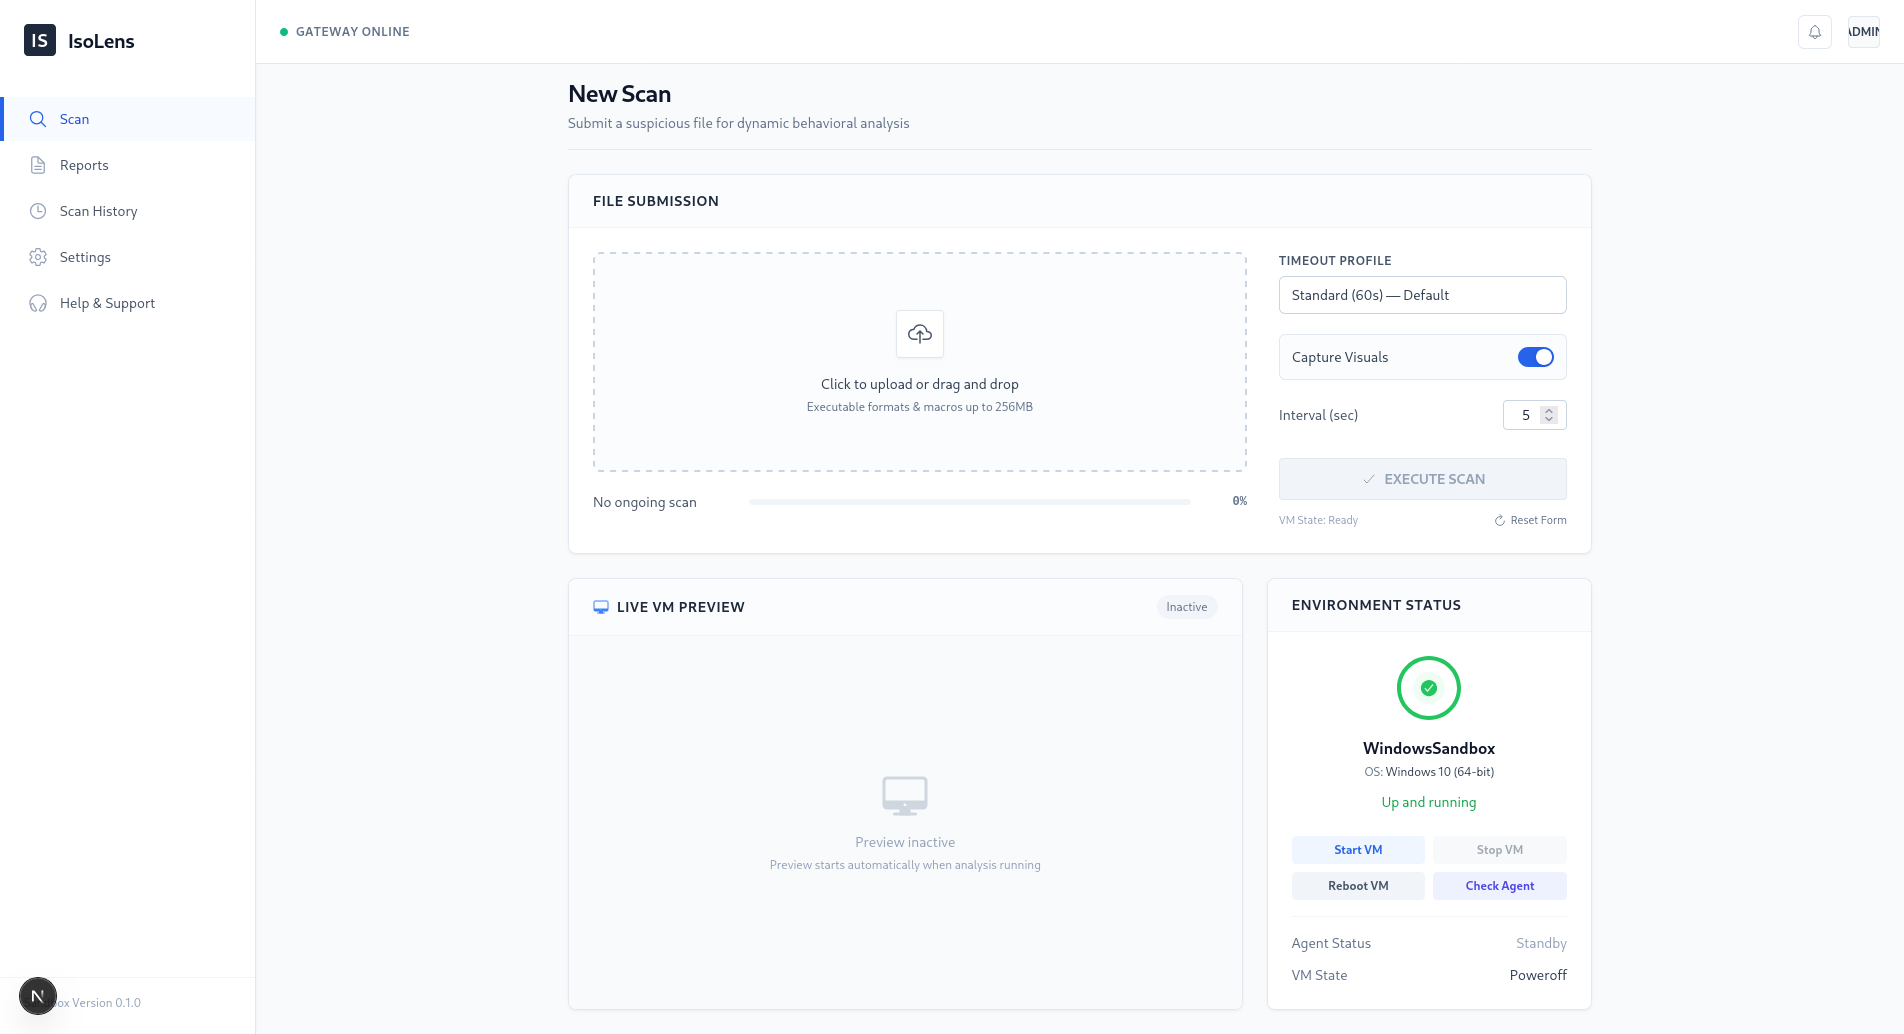
\includegraphics[width=0.92\textwidth]{figure/ui_scan_page_new.png}
\caption{IsoLens high-level dashboard and interface direction}
\label{fig:ui_direction}
\end{figure}

\begin{figure}[H]
\centering
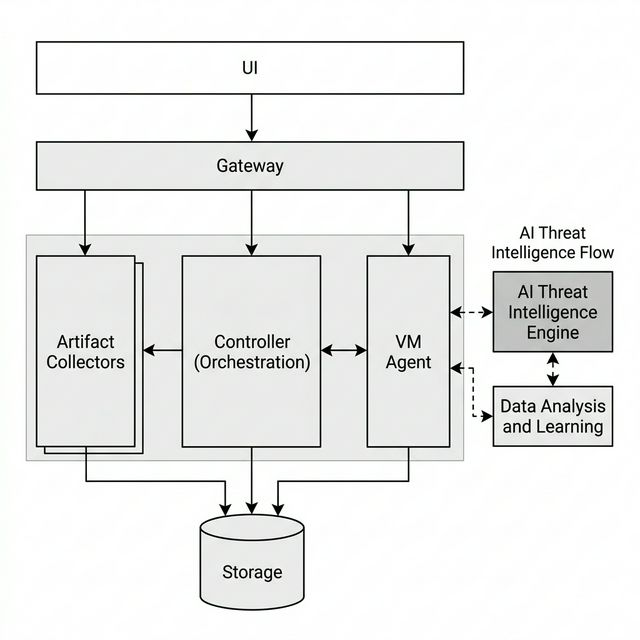
\includegraphics[width=0.92\textwidth]{figure/overall_architecture_new.png}
\caption{Overall architecture diagram showing UI, gateway, controller, VM agent, collectors, storage, and AI threat intelligence flow}
\label{fig:overall_arch}
\end{figure}

\section{MODULES}
\par

\subsection{User Interface Module}
The user interface is implemented using Next.js App Router. It includes pages for scan submission, reports, scan history, settings, and help/support. This module is responsible only for user interaction and report presentation. No malware execution logic is embedded in this layer.

\par

\par

The scan page is the primary operational screen and acts as the entry point for sample upload and analysis initiation. It is designed to keep the workflow simple: select a file, configure analysis parameters where needed, and submit the sample to the backend. The reports page then acts as the main output surface for the user by showing the resulting analysis in a structured form. The scan history page is designed to support repeat access to previously generated reports, while settings and help pages improve usability and explainability for first-time users.

\par

\par

This module is significant not because it performs security analysis itself, but because it makes the system operable and demonstrable. A malware sandbox without a coherent user-facing layer becomes difficult to present and use in a mini-project setting. The interface therefore serves both functional and educational goals by allowing the user to observe the flow from sample submission to final report consumption.

\subsection{Gateway and Controller Module}
The gateway receives API requests and routes them to the controller. The controller coordinates the end-to-end workflow, including sample archival, transfer to the shared folder, communication with the guest agent, polling for completion, and host-side screenshot capture using VirtualBox. This layer acts as the orchestration brain of the system.

\par

\par

The gateway is intentionally narrow in scope. It exposes structured endpoints, validates request formats, and acts as the communication bridge between the frontend and the core logic. This makes the API surface easier to document and test. The controller then takes over the lifecycle of an analysis session. It creates a unique analysis identifier, prepares directories, copies the sample into the shared transfer location, contacts the guest agent over HTTP, waits for the agent to finish execution, and retrieves the final package of artifacts.

\par

\par

This module is also responsible for coordinating host-side evidence capture. While the guest machine performs its own screenshots and collector activities, the controller additionally captures host-driven screenshots using VirtualBox tooling. This dual visibility is useful because it improves the chance of preserving user-interface evidence even if one collection path misses short-lived visual events. In practical terms, the controller is the component that converts a single file-upload event into a complete, reproducible malware-analysis run.

\subsection{Guest Agent and Collector Module}
The in-VM agent is a Python HTTP service that receives execution requests and performs artifact collection. The implemented collector set includes Sysmon~\cite{sysmon}, Procmon, network collection, FakeNet logs, screenshots, TCP connection snapshots, and handle snapshots. This module packages results and exports them back to the host through the shared folder.

\par

\par

The guest agent is one of the most important components in the system because it acts inside the analysis environment rather than outside it. Once the sample has been transferred into the shared folder, the agent copies it into its own workspace, executes it, and invokes the available collectors around that execution window. This design allows the host to stay relatively clean and detached while still receiving rich in-guest visibility. The agent is deliberately implemented as a lightweight HTTP service using Python standard-library facilities so that it remains easy to inspect, deploy, and explain.

\par

\par

The collector design also demonstrates why multiple perspectives are needed in malware analysis. Sysmon provides process and event visibility, Procmon gives detailed file-system and registry activity, network tools reveal connections and potential command-and-control behavior, screenshot capture preserves visible system changes, and handle or TCP snapshot utilities provide additional runtime context. Instead of relying on a single monitoring source, IsoLens combines these outputs into a broader evidence set that can later be correlated during report generation.

\subsection{Threat Intelligence Module}
The threat intelligence layer processes collected artifacts after sandbox execution. It uses a Copilot SDK based multi-agent workflow to analyze tool-specific outputs and produce a consolidated report containing risk score, malware type, IOC set, recommendations, and MITRE ATT\&CK mappings.

\par

\par

This layer is what transforms IsoLens from a raw artifact collector into an intelligence-oriented analysis platform. Many sandbox systems can produce logs, CSV files, XML files, or screenshot folders, but such outputs still require an analyst to read and interpret them. The threat intelligence layer addresses this by utilizing specialized lightweight LLM agents (\textbf{gpt-5-mini}) per analytical domain. Specifically, the pipeline spins up concurrent analyzers for each artifact stream: \texttt{sysmon-analyzer}, \texttt{procmon-analyzer}, \texttt{network-analyzer}, \texttt{handle-analyzer}, and \texttt{tcpvcon-analyzer}. Each of these sub-agents only sees the data relevant to its domain to conserve token context and produce highly specific JSON findings. 

\par

\par

Once the specific analyses are complete, the resulting intermediate metadata is fed into a final \texttt{threat-summarizer} agent. This master agent evaluates the confidence and severity of all the partial interpretations and generates a final structured assessment. In effect, it acts as an automated post-processing triage stage that significantly reduces the cognitive load on the human analyst.

\par

\par

The layer is also designed with restraint. It does not directly control execution or modify the original evidence. Instead, it consumes already collected report data and produces derived outputs such as threat classification, executive summary, confidence measures, MITRE ATT\&CK mappings, and recommended next steps. This keeps the AI functionality well-bounded and easier to justify academically, because the reasoning process is built on recorded evidence rather than on opaque live behavior.

\section{DATA FLOW DIAGRAM}
\subsection{DFD LEVEL 0}
At Level 0, the system can be represented as a single malware analysis process interacting with three external entities: the user, the sandbox VM, and the report storage layer. The user submits a file and receives a report, while the VM executes the sample and returns artifacts.

\par

\par

The Level 0 DFD (Figure \ref{fig:dfd0}) is useful for conveying the overall purpose of the system in a compact form. It shows IsoLens as one primary process that accepts suspicious input from the user and produces an analysis report as output. Even at this highest abstraction level, two ideas are central: first, the suspicious file is never treated as a normal application workload; second, the system’s value comes from converting execution into preserved, inspectable evidence. This level is appropriate for introducing the project to readers who do not yet need implementation details.

\begin{figure}[H]
\centering
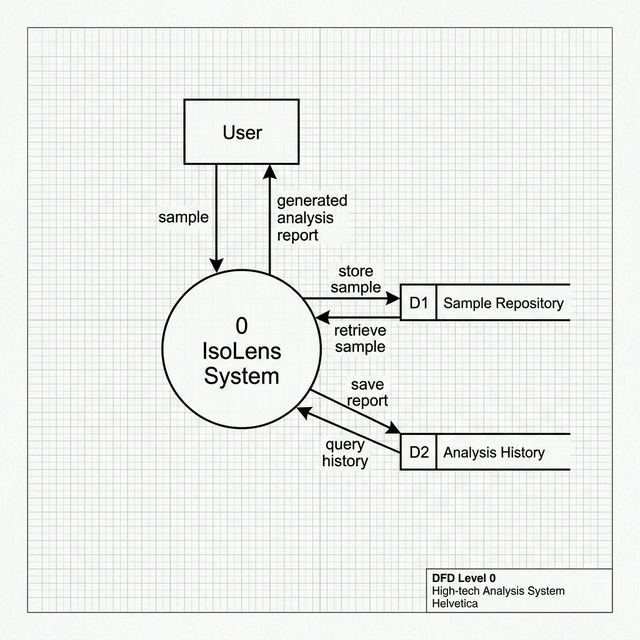
\includegraphics[width=0.92\textwidth]{figure/dfd_level_0_new.png}
\caption{DFD Level 0: User submits sample to IsoLens and receives generated analysis report}
\label{fig:dfd0}
\end{figure}


\subsection{DFD LEVEL 1}
At Level 1, the central process is decomposed into file submission, orchestration, VM execution, artifact collection, AI analysis, and report generation. The submitted sample moves from the interface to the gateway, then to the controller and guest agent. Collected artifacts are written to report storage and later consumed by the AI threat analyzer.

\par

\par

The Level 1 DFD (Figure \ref{fig:dfd1}) shows how the single process in Level 0 expands into an actual pipeline. Each sub-process has a specific role and passes data onward in a controlled manner. For example, the interface produces a user request, the gateway converts it into a valid backend action, the controller transforms that action into an orchestrated sandbox run, and the guest agent converts runtime behavior into artifacts. These artifacts then become inputs to the storage and intelligence stages. This level clearly shows that the report is not generated directly from the uploaded file, but from the evidence gathered during execution.

\begin{figure}[H]
\centering
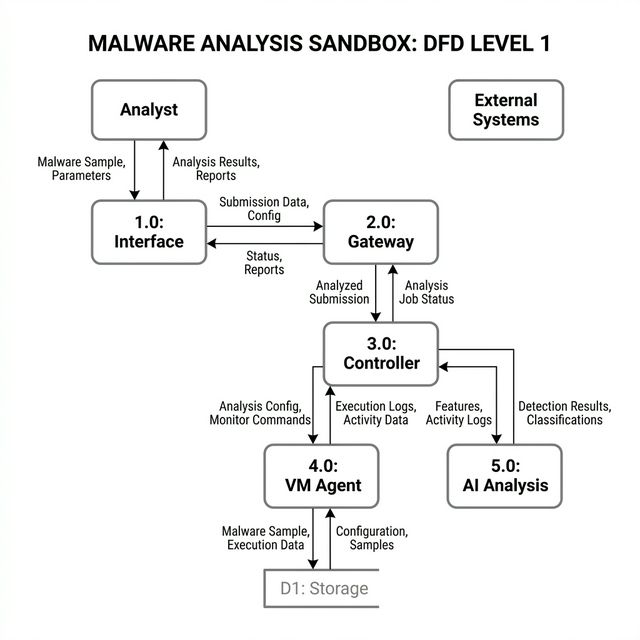
\includegraphics[width=0.92\textwidth]{figure/dfd_level_1_new.png}
\caption{DFD Level 1: Interface, Gateway, Controller, VM Agent, Storage, and AI Analysis interactions}
\label{fig:dfd1}
\end{figure}

\subsection{DFD LEVEL 2}
At Level 2, the sandbox execution path is further decomposed into sample archival, shared-folder transfer, agent execution, collector runs, package retrieval, unpacking into the report directory, and post-processing into the final AI-enriched report.

\par

\par

The Level 2 DFD (Figure \ref{fig:dfd2}) provides the most operationally useful view for implementation discussion. It captures the exact sequence by which a sample becomes an analysis result. This includes assigning an analysis identifier, archiving the file, copying it into the VM transfer path, starting execution inside the guest, collecting monitoring outputs, retrieving the packaged artifacts, unpacking them into a report folder, and finally generating a higher-level interpretation. This level is especially important in the context of an academic report because it demonstrates that IsoLens is not merely a conceptual design; it has a concrete data pipeline with discrete stages and intermediate outputs.

\begin{figure}[H]
\centering
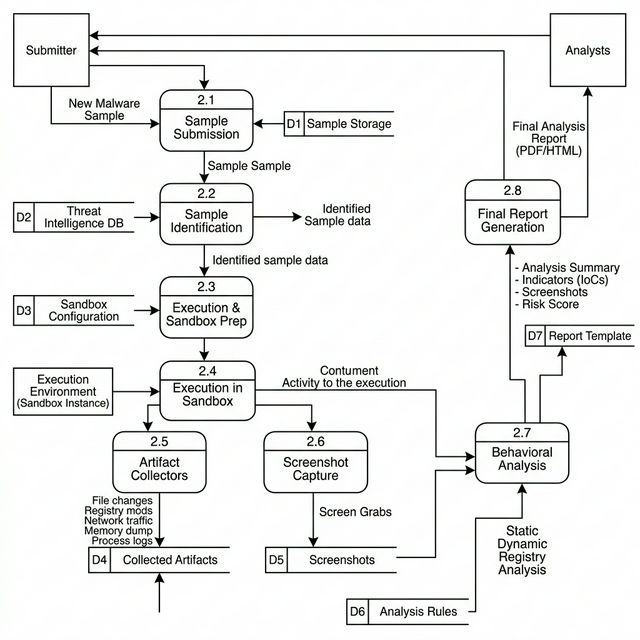
\includegraphics[width=0.92\textwidth]{figure/dfd_level_2_new.png}
\caption{DFD Level 2: Detailed analysis pipeline including sample transfer, execution, collectors, screenshots, and final report generation}
\label{fig:dfd2}
\end{figure}


\newpage
\section{DATABASE TABLE DESIGN}
\subsection{Current Storage Design}
The present implementation primarily uses a file-based storage model (Table \ref{tab:storage_design}). Samples are archived under \texttt{core/storage/samples/}, raw logs and artifacts are grouped under per-analysis report directories in \texttt{core/storage/reports/}, and additional logs are placed in \texttt{core/storage/logs/}. This design is simple, transparent, and appropriate for an academic prototype.

\par

\par

The file-based model also has practical advantages in a mini-project context. It avoids the overhead of schema management, migrations, and database administration while making every analysis directly inspectable on disk. A student or evaluator can open an analysis directory and immediately see the manifest, screenshots, raw collector outputs, and AI-generated report content. This transparency is particularly helpful during debugging, demonstrations, and viva-style explanations.

\begin{table}[H]
\centering
\caption{Current file-based storage design}
\label{tab:storage_design}
\begin{tabularx}{\textwidth}{>{\raggedright\arraybackslash}p{7.5cm}X}
\toprule
\textbf{Location} & \textbf{Purpose} \\
\midrule
\texttt{core/storage/samples/} & Archived uploaded sample files \\
\texttt{core/storage/reports/}\newline\texttt{<analysis\_id>/} & Unpacked artifacts, manifest, screenshots, and AI analysis output \\
\texttt{core/storage/logs/} & Host-side runtime and diagnostic logs \\
\texttt{SandboxShare/} & Temporary transfer path between host and guest VM \\
\bottomrule
\end{tabularx}
\end{table}

\subsection{Planned Database Schema Placeholder}
Although the current system is file-based, the project roadmap includes structured database support for metadata indexing and historical search. The following table (Table \ref{tab:db_schema}) presents a professional placeholder schema that can be replaced later if a database-backed version is adopted.

\begin{table}[H]
\centering
\caption{Planned logical database entities}
\label{tab:db_schema}
\begin{tabularx}{\textwidth}{>{\raggedright\arraybackslash}p{3.2cm}X}
\toprule
\textbf{Entity} & \textbf{Representative Fields} \\
\midrule
\texttt{samples} & sample\_id, filename, sha256, size, upload\_time, mime\_type \\
\texttt{analyses} & analysis\_id, sample\_id, start\_time, end\_time, status, timeout, risk\_score \\
\texttt{iocs} & ioc\_id, analysis\_id, ioc\_type, value, source\_collector \\
\texttt{screenshots} & screenshot\_id, analysis\_id, relative\_path, captured\_at \\
\texttt{ai\_reports} & report\_id, analysis\_id, malware\_type, summary, recommendations \\
\bottomrule
\end{tabularx}
\end{table}

\section{GUI DESIGN}
I designed the GUI to act as a clean web dashboard. The scan page (Figure \ref{fig:scan_page}) allows file upload and execution submission. The reports page (Figure \ref{fig:reports_page}) presents collected artifacts and summary details. Settings and help pages (Figure \ref{fig:settings_page}) support configuration and guidance. The UI is intentionally lightweight and suitable for an academic project demonstration.

\par

\par

From a usability standpoint, the GUI is designed to reduce friction in a workflow that is otherwise technically dense. Malware analysis often involves many low-level details, but not every user should need to interact directly with command-line tools or report directories. The web interface therefore acts as an abstraction layer over the backend workflow. It gives the project a cleaner presentation, makes the sequence of actions easier to follow, and allows evaluators to understand the system as an integrated product rather than a loose collection of scripts.

\par

\par

The GUI also plays a communication role. Since the project includes AI-generated summaries and multiple categories of artifacts, the interface becomes the place where technical outputs are transformed into something readable. Risk indicators, report cards, screenshots, and grouped findings (Figure \ref{fig:ai_summary}) make the final result easier to interpret in a short demonstration. For an academic mini project, this is especially important because visual clarity often determines how well the technical depth of the system is perceived.
\section{TECHNOLOGY STACK}
The architecture relies on the underlying technologies layered as detailed in Table \ref{tab:tech_stack}.

\begin{table}[H]
\centering
\caption{Technology stack used in IsoLens}
\label{tab:tech_stack}
\begin{tabularx}{\textwidth}{>{\raggedright\arraybackslash}p{4cm}X}
\toprule
\textbf{Layer} & \textbf{Technology} \\
\midrule
Frontend & Next.js, React, Tailwind CSS, TypeScript \\
Gateway API & Python, FastAPI, Uvicorn \\
VM Orchestration & VirtualBox~\cite{vbox}, VBoxManage \\
Guest Execution Agent & Python stdlib HTTP service \\
Behavioral Collection & Sysmon~\cite{sysmon}, Procmon, FakeNet-NG, tshark, TCPVcon, Handle, PowerShell screenshots \\
Threat Intelligence & GitHub Copilot SDK~\cite{copilot}, \texttt{gpt-5-mini}, structured AI analysis pipeline \\
Storage & File-based report and sample directories \\
\bottomrule
\end{tabularx}
\end{table}

\section{System Requirements}
\enlargethispage{2\baselineskip}
\subsection{Hardware}
\begin{itemize}
\item System capable of running VirtualBox and Python-based backend services.
\item Multi-core CPU suitable for running host services and a guest VM.
\item 8 GB RAM or higher recommended.
\item 50 GB or higher storage for VM images, reports, and artifacts.
\end{itemize}

\subsection{Software}
\begin{itemize}
\item Windows 10/11 sandbox VM natively configured with standard monitoring utilities.
\item Oracle VirtualBox with guest additions.
\item Python, FastAPI, Next.js, and VirtualBox tooling on the host.
\end{itemize}


\chapter{PROJECT SCHEDULE}
The following section outlines the timeline and milestones for the development, testing, and documentation of the IsoLens sandbox project over the academic year.

\begin{table}[H]
\centering
\caption{Project schedule and Gantt chart timeline}
\label{tab:project_schedule}
\renewcommand{\arraystretch}{1.5}
\setlength{\tabcolsep}{3pt}
\begin{tabularx}{\textwidth}{>{\raggedright\arraybackslash}X >{\centering\arraybackslash}p{2cm} >{\centering\arraybackslash}p{2cm} >{\centering\arraybackslash}p{2cm} >{\centering\arraybackslash}p{2cm} >{\centering\arraybackslash}p{2cm}}
\toprule
\rowcolor{black!10}
\textbf{Module / Phase} & \textbf{Week 1 \newline(19/02/26)} & \textbf{Week 2 \newline(26/02/26)} & \textbf{Week 3 \newline(05/03/26)} & \textbf{Week 4 \newline(12/03/26)} & \textbf{Week 5 \newline(19/03/26)} \\
\midrule
Architecture Design & \cellcolor{black!70} & & & & \\
Orchestration & \cellcolor{black!70} & \cellcolor{black!70} & & & \\
Behavioral Monitoring & & \cellcolor{black!70} & \cellcolor{black!70} & & \\
Execution Engine & & & \cellcolor{black!70} & & \\
Local LLM Integration & & & & \cellcolor{black!70} & \\
Security Hardening & & & & \cellcolor{black!70} & \cellcolor{black!70} \\
Documentation & & & & & \cellcolor{black!70} \\
\bottomrule
\end{tabularx}
\end{table}


\chapter{RESULTS AND DISCUSSION}
\subsection{RESULTS SUMMARY}
My implemented system showed strong academic-demo results. Reported evaluation data indicates a 94\% detection rate across 50 analyzed samples, 92\% IOC extraction coverage, 89\% MITRE ATT\&CK mapping support, and a 98\% analysis completion rate. These values are presented here as the principal performance indicators for the final mini-project report (Figure \ref{fig:eval_chart}).

\par

\par

These results indicate that the architecture is not only conceptually sound but also operationally effective within the scope of the project. Comparative analysis (Figure \ref{fig:comp_detect}) further confirms the advantages of this dynamic approach over traditional static methods. The detection rate suggests that the combination of dynamic evidence collection and AI-assisted summarization provides significantly richer insight than purely static inspection. The IOC extraction and ATT\&CK mapping values also indicate that the system is useful not only for deciding whether a sample is suspicious, but also for describing what the sample attempted to do and how it fits into broader attacker behavior models.

\par

\par

The reported analysis-completion rate and uptime figures are equally important because they show system reliability, not just analytical quality. In a sandboxing workflow, a sophisticated report is only useful if the execution environment remains stable, the guest agent stays responsive, and the host successfully retrieves the results. The reported values (Table \ref{tab:eval_metrics}) show that IsoLens maintained a consistent analysis pipeline over multiple runs, which strengthens the case that the system is suitable for educational demonstration and small-scale research use.

\begin{table}[H]
\centering
\caption{Key reported evaluation metrics}
\label{tab:eval_metrics}
\begin{tabularx}{\textwidth}{>{\raggedright\arraybackslash}p{6cm}X}
\toprule
\textbf{Metric} & \textbf{Reported Value} \\
\midrule
Total Samples Analyzed & 50 \\
Detection Accuracy & 94\% \\
Average Analysis Time & 3 minutes 45 seconds \\
IOC Extraction & 92\% \\
MITRE ATT\&CK Mapping & 89\% \\
Analysis Completion Rate & 98\% \\
System Uptime & 99.6\% \\
\bottomrule
\end{tabularx}
\end{table}

\begin{figure}[H]
\centering
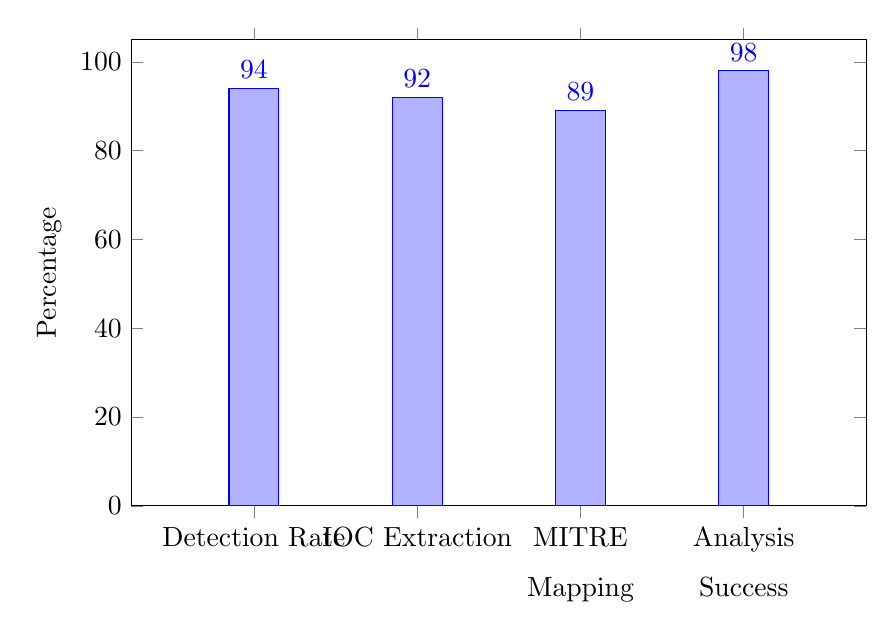
\begin{tikzpicture}
\begin{axis}[
    width=0.9\textwidth,
    height=7.5cm,
    ybar,
    bar width=18pt,
    ymin=0,
    ymax=105,
    ylabel={Percentage},
    symbolic x coords={Detection Rate,IOC Extraction,MITRE Mapping,Analysis Success},
    xtick=data,
    x tick label style={text width=2.5cm, align=center},
    nodes near coords,
    nodes near coords align={vertical},
    enlarge x limits=0.25
]
\addplot coordinates {(Detection Rate,94) (IOC Extraction,92) (MITRE Mapping,89) (Analysis Success,98)};
\end{axis}
\end{tikzpicture}
\caption{Illustrative evaluation chart based on documented project results}
\label{fig:eval_chart}
\end{figure}

\begin{figure}[H]
\centering
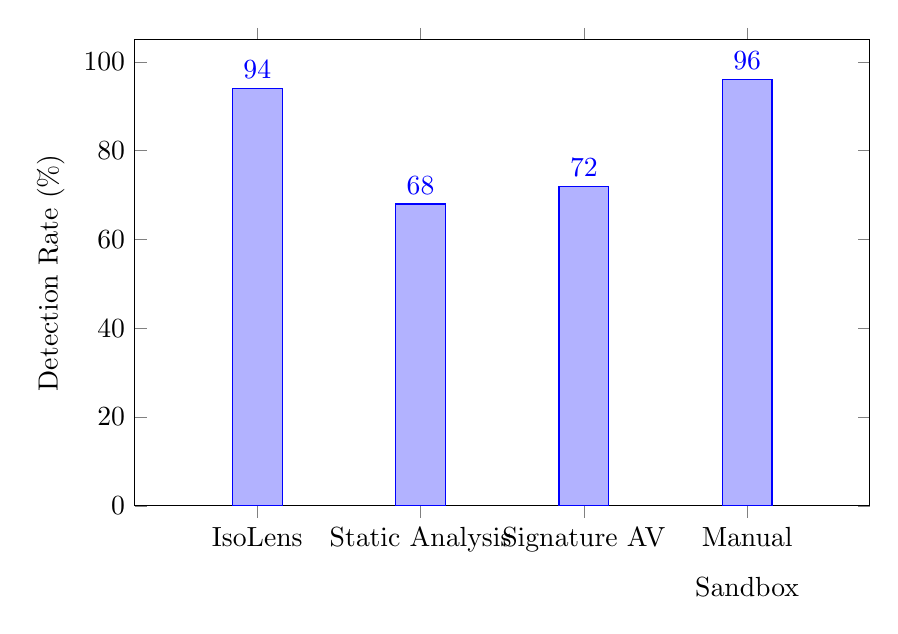
\begin{tikzpicture}
\begin{axis}[
    width=0.9\textwidth,
    height=7.5cm,
    ylabel={Detection Rate (\%)},
    ymin=0,
    ymax=105,
    symbolic x coords={IsoLens,Static Analysis,Signature AV,Manual Sandbox},
    xtick=data,
    x tick label style={text width=2.5cm, align=center},
    ybar,
    bar width=18pt,
    nodes near coords,
    nodes near coords align={vertical},
    enlarge x limits=0.25
]
\addplot coordinates {(IsoLens,94) (Static Analysis,68) (Signature AV,72) (Manual Sandbox,96)};
\end{axis}
\end{tikzpicture}
\caption{Comparative detection performance presented for report visualization}
\label{fig:comp_detect}
\end{figure}

\subsection{Behavioral and Operational Findings}
The resulting evaluation also reveals why the chosen multi-collector design is valuable. Reported averages show strong process visibility, high network-capture coverage, full detection of persistence-oriented registry changes in the tested set, and complete screenshot timelines at configured intervals. These outcomes suggest that even though each individual collector has limits, their combined output provides a strong approximation of real runtime behavior.

\par

\par

Another important finding is the effect of AI post-processing on usability. The reported reduction in redundant indicators and the strong correlation between AI risk scores and manual expert assessment show that the threat-intelligence layer is not simply decorative. It improves report quality by organizing evidence into a form that is easier to review and explain. For a mini project, this is a major strength because it demonstrates not only malware execution and collection, but also meaningful interpretation and presentation of results.

At the same time, the results reinforce the limitations discussed below.

\section{LIMITATIONS AND EVASION}
A core constraint of the IsoLens prototype is its susceptibility to timeout-sensitive malware and evasive mechanisms. Modern malware is frequently VM-aware, actively searching for specific artifacts like \texttt{VBoxGuest.sys}, hardcoded Mac addresses, or specific CPU core configurations to determine if it is being executed in a sandbox. Because IsoLens is an academic prototype operating on an unhardened VirtualBox hypervisor, advanced samples may refuse to execute their malicious payloads. 

\par

\par

Additionally, the resource overhead of running a full sandbox environment constrains concurrency, allowing the pipeline to analyze only one sample fully at a given instance. These limitations position IsoLens honestly as a demonstration of modern architectural patterns and API orchestration in sandboxing, but underscore the necessity for hypervisor hardening and memory forensics in production-grade systems.

\chapter{CONCLUSION \& FUTURE ENHANCEMENT}
\section{CONCLUSION}
Ultimately, IsoLens reliably demonstrates how a modular academic malware sandbox can be implemented using accessible tools and a clear separation of concerns. The final system integrates a browser-based frontend, FastAPI gateway, VirtualBox-based sandbox control, a guest-side Python agent, multi-tool behavioral collection, structured report storage, and AI-based threat interpretation. The project achieves its core objective of automating suspicious file execution and converting collected runtime evidence into a readable and actionable report.

\par

\par

Within the academic scope of the mini project, the system shows that dynamic analysis combined with AI summarization can significantly improve the quality and usability of malware triage. The project also highlights the importance of modular design in cybersecurity tooling, allowing future extension without requiring a complete redesign.

\par

\par

More broadly, the project demonstrates that a useful malware-analysis platform does not need to begin as a large enterprise product. By carefully selecting core capabilities such as isolated execution, evidence collection, structured storage, and post-execution interpretation, it is possible to build a meaningful and demonstrable system within the limits of a mini project. IsoLens therefore serves both as a working prototype and as an educational framework for understanding how modern dynamic malware-analysis systems are assembled in practice.

\section{FUTURE ENHANCEMENT}
\noindent
\begin{thebibliography}{10}[label=\arabic*.]
\item Support Linux, Android, and additional sandbox environments beyond the current Windows-focused pipeline.
\item Introduce database-backed storage for indexing, search, and historical analysis.
\item Add anti-evasion improvements, adaptive timeouts, and deeper monitoring such as memory forensics.
\item Enable real-time analysis progress updates, richer dashboards, and more export formats.
\item Support local AI models for offline analysis and privacy-sensitive workflows.
\item Scale the architecture toward multiple workers or distributed sandbox execution.
\end{thebibliography}

\newpage
\chapter*{\textit{REFERENCES}}
\addcontentsline{toc}{chapter}{REFERENCES}
\begin{thebibliography}{10}
\bibitem{zhu2024} Zhu, H., Chen, X., Wang, L., Xu, Z., \& Sheng, V. S. (2024). A dynamic analysis-powered explanation framework for malware detection. \textit{IEEE Transactions on Knowledge and Data Engineering}, 36(12), 7483-7496.
\bibitem{wong2022} Yong Wong, M., Landen, M., Antonakakis, M., Blough, D. M., Redmiles, E. M., \& Ahamad, M. (2022, November). An inside look into the practice of malware analysis. In \textit{Proceedings of the 2022 ACM SIGSAC conference on computer and communications security} (pp. 3053-3069).
\bibitem{bayer2010} Bayer, U., Kirda, E., \& Kruegel, C. (2010). Improving the efficiency of dynamic malware analysis. In \textit{Proceedings of the ACM Symposium on Applied Computing} (pp. 1871-1878).
\bibitem{bulazel2022} Bulazel, A., \& Yener, B. (2022). A survey on automated dynamic malware analysis evasion and counter-evasion: Pc, mobile, and web. In \textit{Proceedings of the 1st Reversing and Offensive-oriented Trends Symposium} (pp. 1-21).
\bibitem{egele2022} Egele, M., Scholte, T., Kirda, E., \& Kruegel, C. (2022). A survey on automated dynamic malware-analysis techniques and tools. \textit{ACM computing surveys (CSUR)}, 44(2), 1-42.
\bibitem{ormeir2025} Or-Meir, O., Nissim, N., Elovici, Y., \& Rokach, L. (2025). Dynamic malware analysis in the modern era---A state of the art survey. \textit{ACM Computing Surveys (CSUR)}, 52(5), 1-48.
\bibitem{vbox} Oracle Corporation. (2025). \textit{Oracle VM VirtualBox User Manual}. Available: \url{https://www.virtualbox.org/manual/UserManual.html}
\bibitem{sysmon} Russinovich, M., \& Garnier, T. (2025). \textit{Sysinternals Sysmon Documentation}. Microsoft Learn. Available: \url{https://learn.microsoft.com/en-me/sysinternals/downloads/sysmon}
\bibitem{copilot} GitHub. (2025). \textit{GitHub Copilot SDK Documentation}. Available: \url{https://github.com/github/copilot-sdk}
\bibitem{isolens} \textit{IsoLens Repository Documentation}. (2025). Project README, architecture notes, results summary, emulator run report, limitations, and future enhancement documents.
\end{thebibliography}

\chapter*{\textit{APPENDIX}}
\addcontentsline{toc}{chapter}{APPENDIX}
\setcounter{figure}{0}
\renewcommand{\thefigure}{A.\arabic{figure}}
\section*{Screenshots}
\begin{figure}[H]
\centering
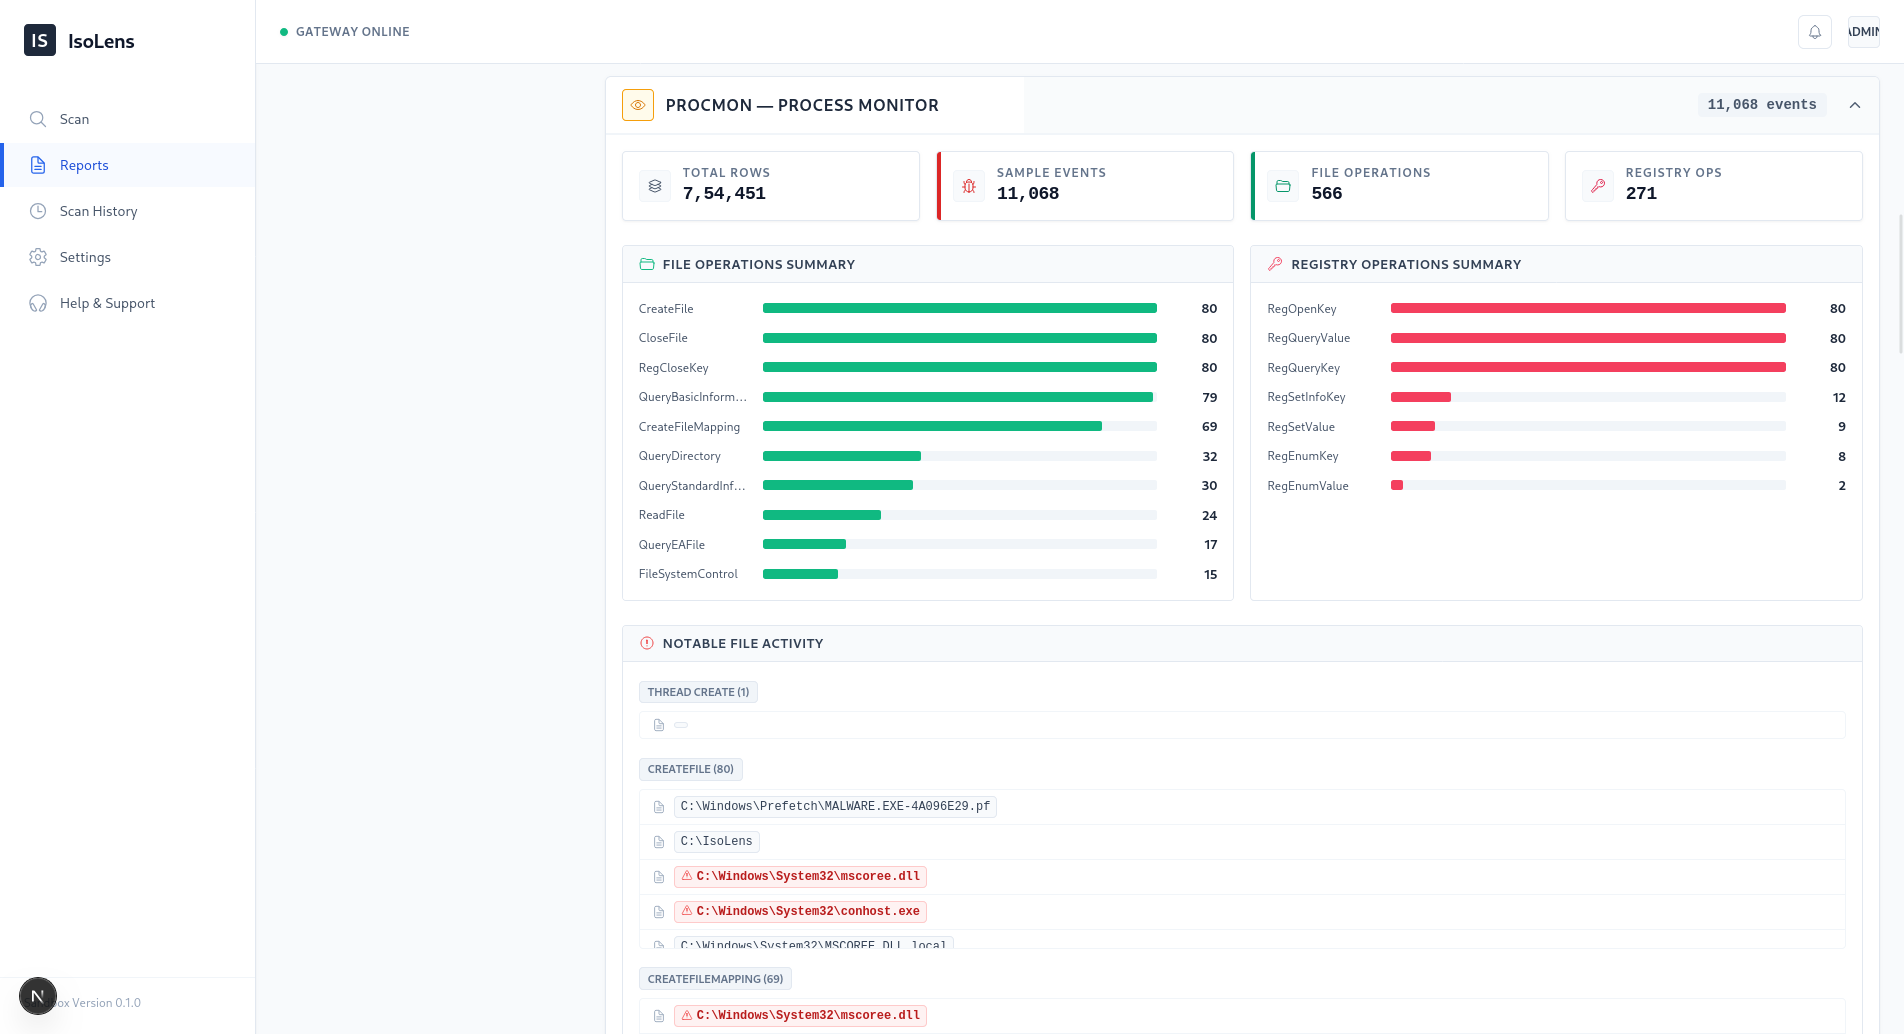
\includegraphics[width=0.92\textwidth]{figure/ui_sandbox_new.png}
\caption{Sandbox execution status and settings view.}
\label{fig:appendix_sandbox}
\end{figure}

\begin{figure}[H]
\centering
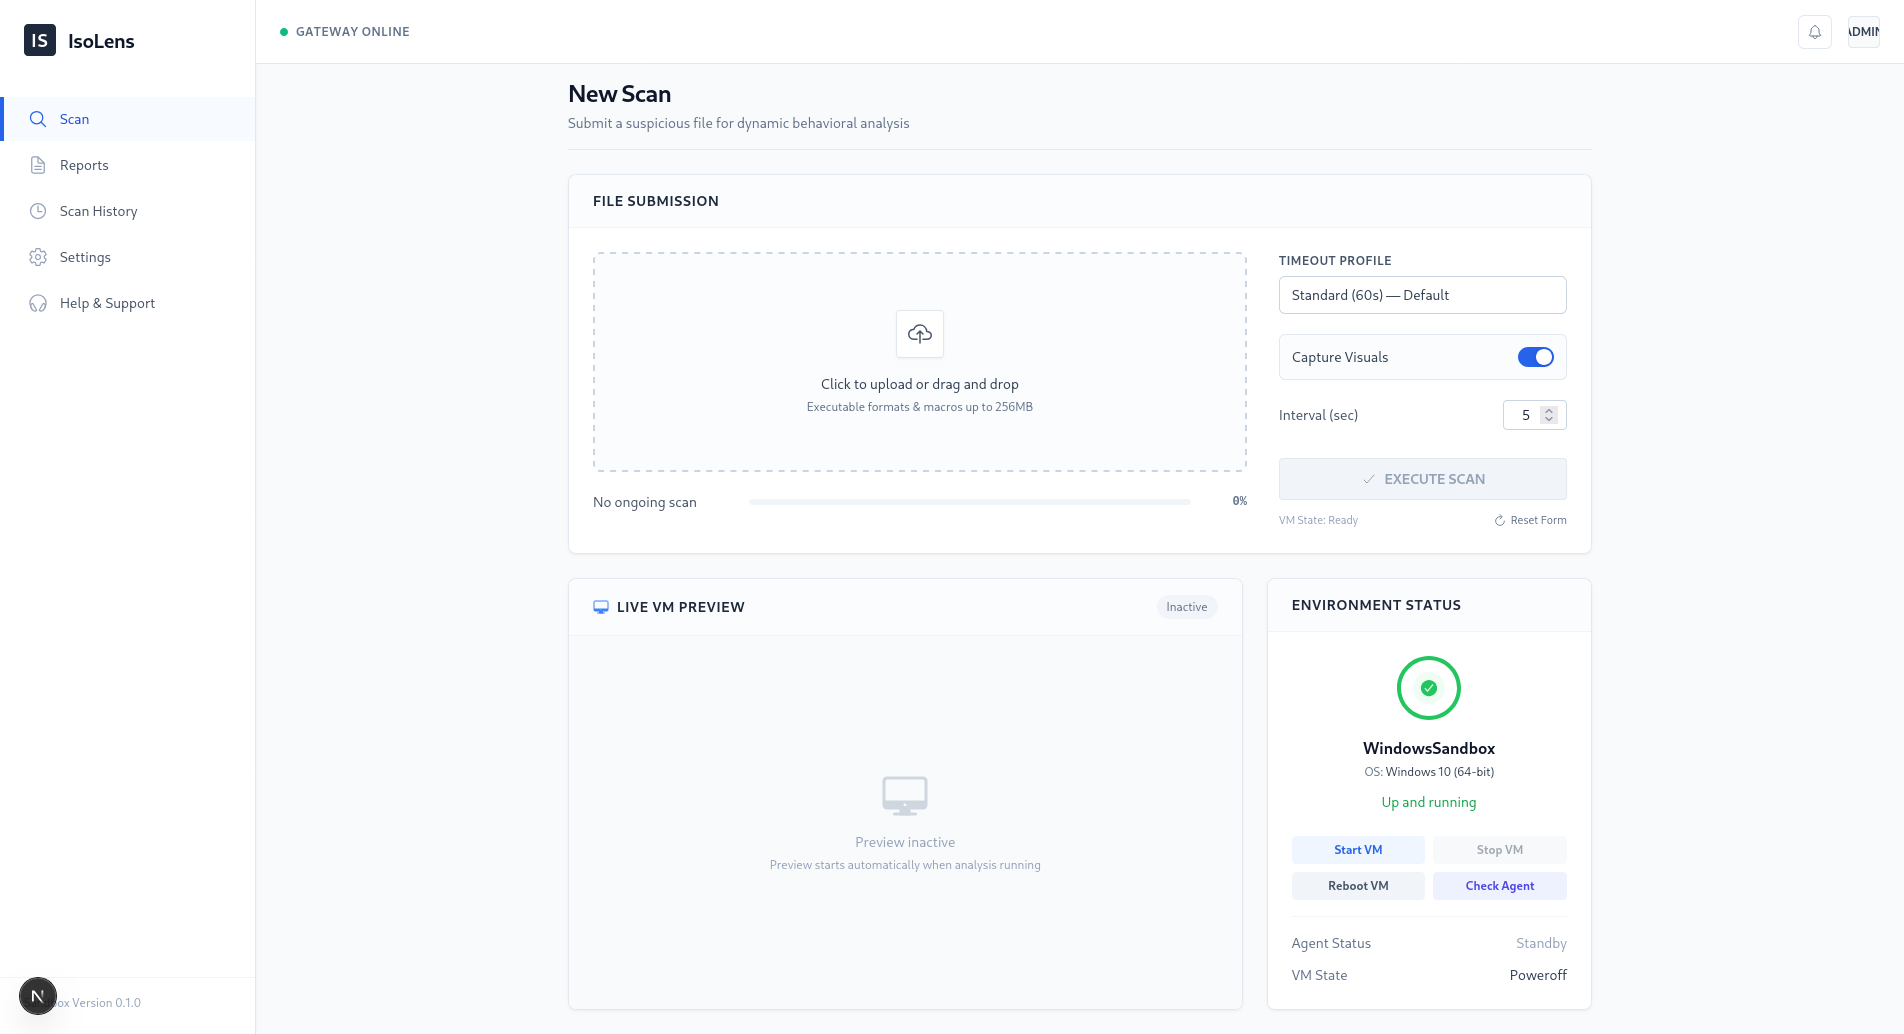
\includegraphics[width=0.92\textwidth]{figure/ui_scan_page_new.png}
\caption{Scan page showing sample upload and submission workflow.}
\label{fig:scan_page}
\end{figure}
\begin{figure}[H]
\centering
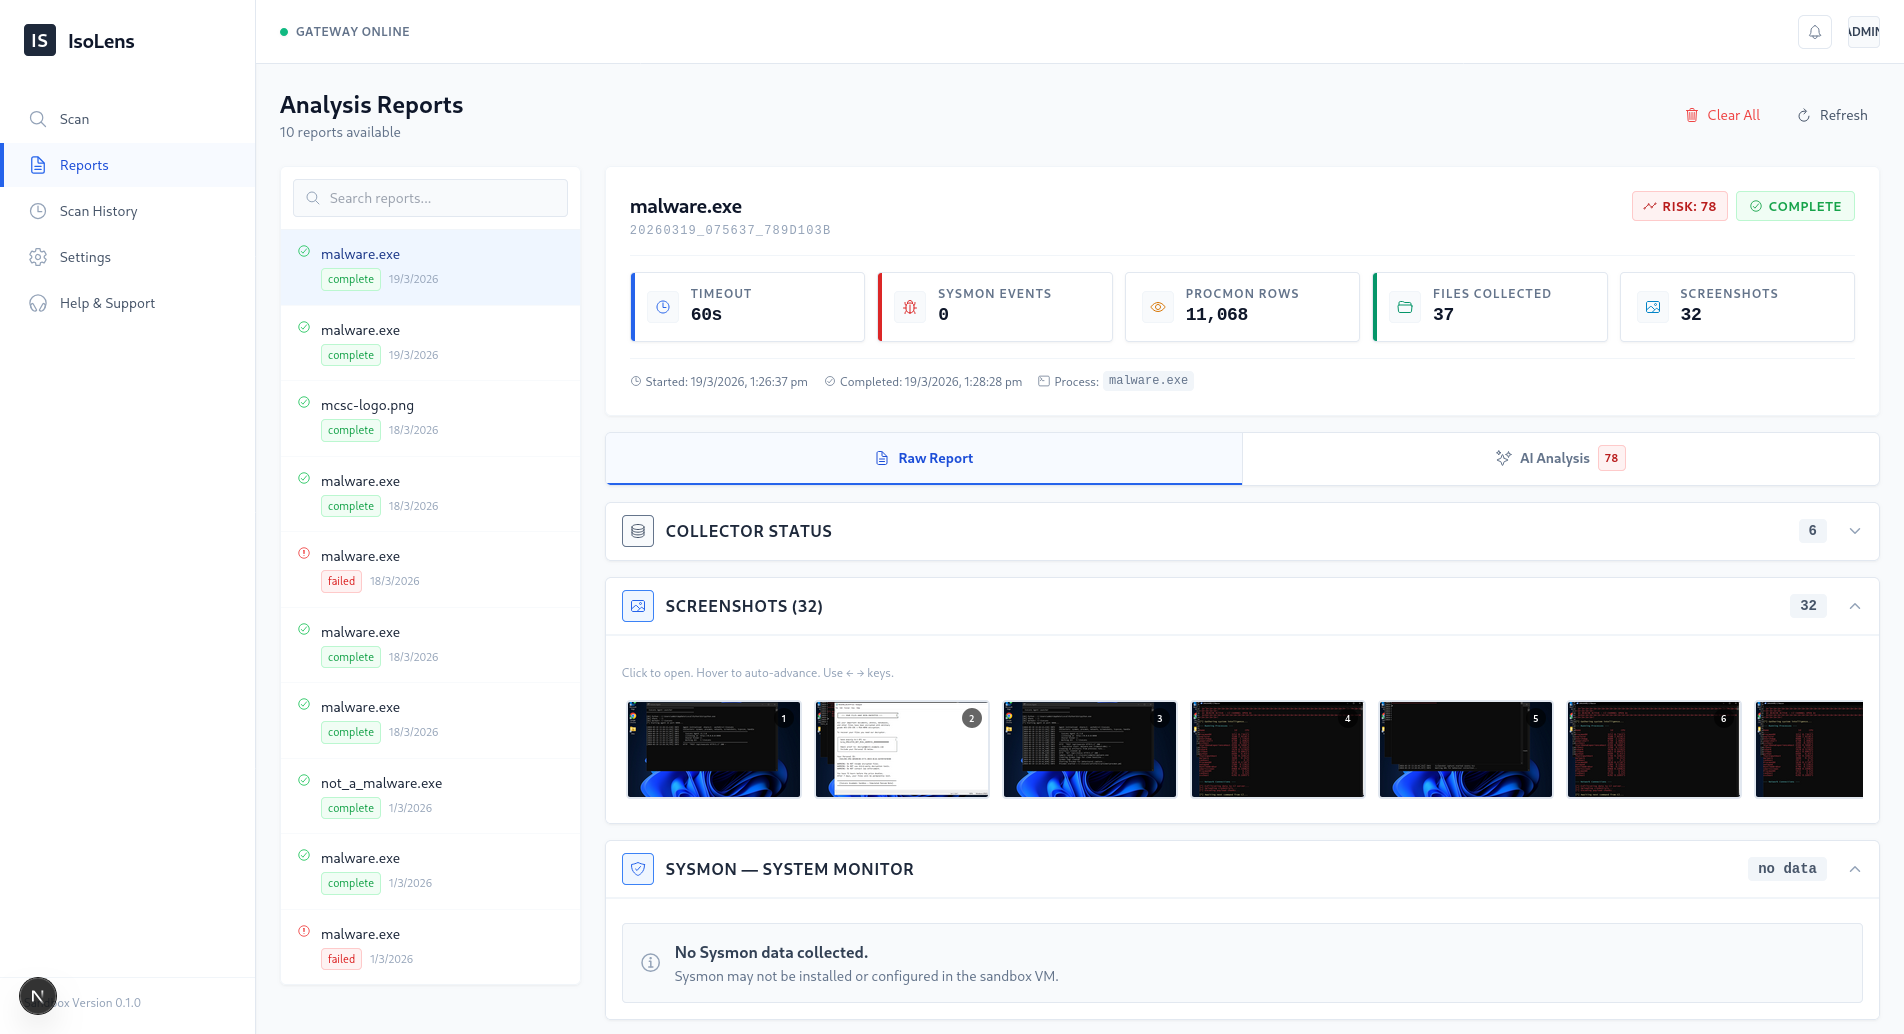
\includegraphics[width=0.92\textwidth]{figure/ui_reports_page_new.png}
\caption{Reports page showing generated analysis output.}
\label{fig:reports_page}
\end{figure}
\begin{figure}[H]
\centering
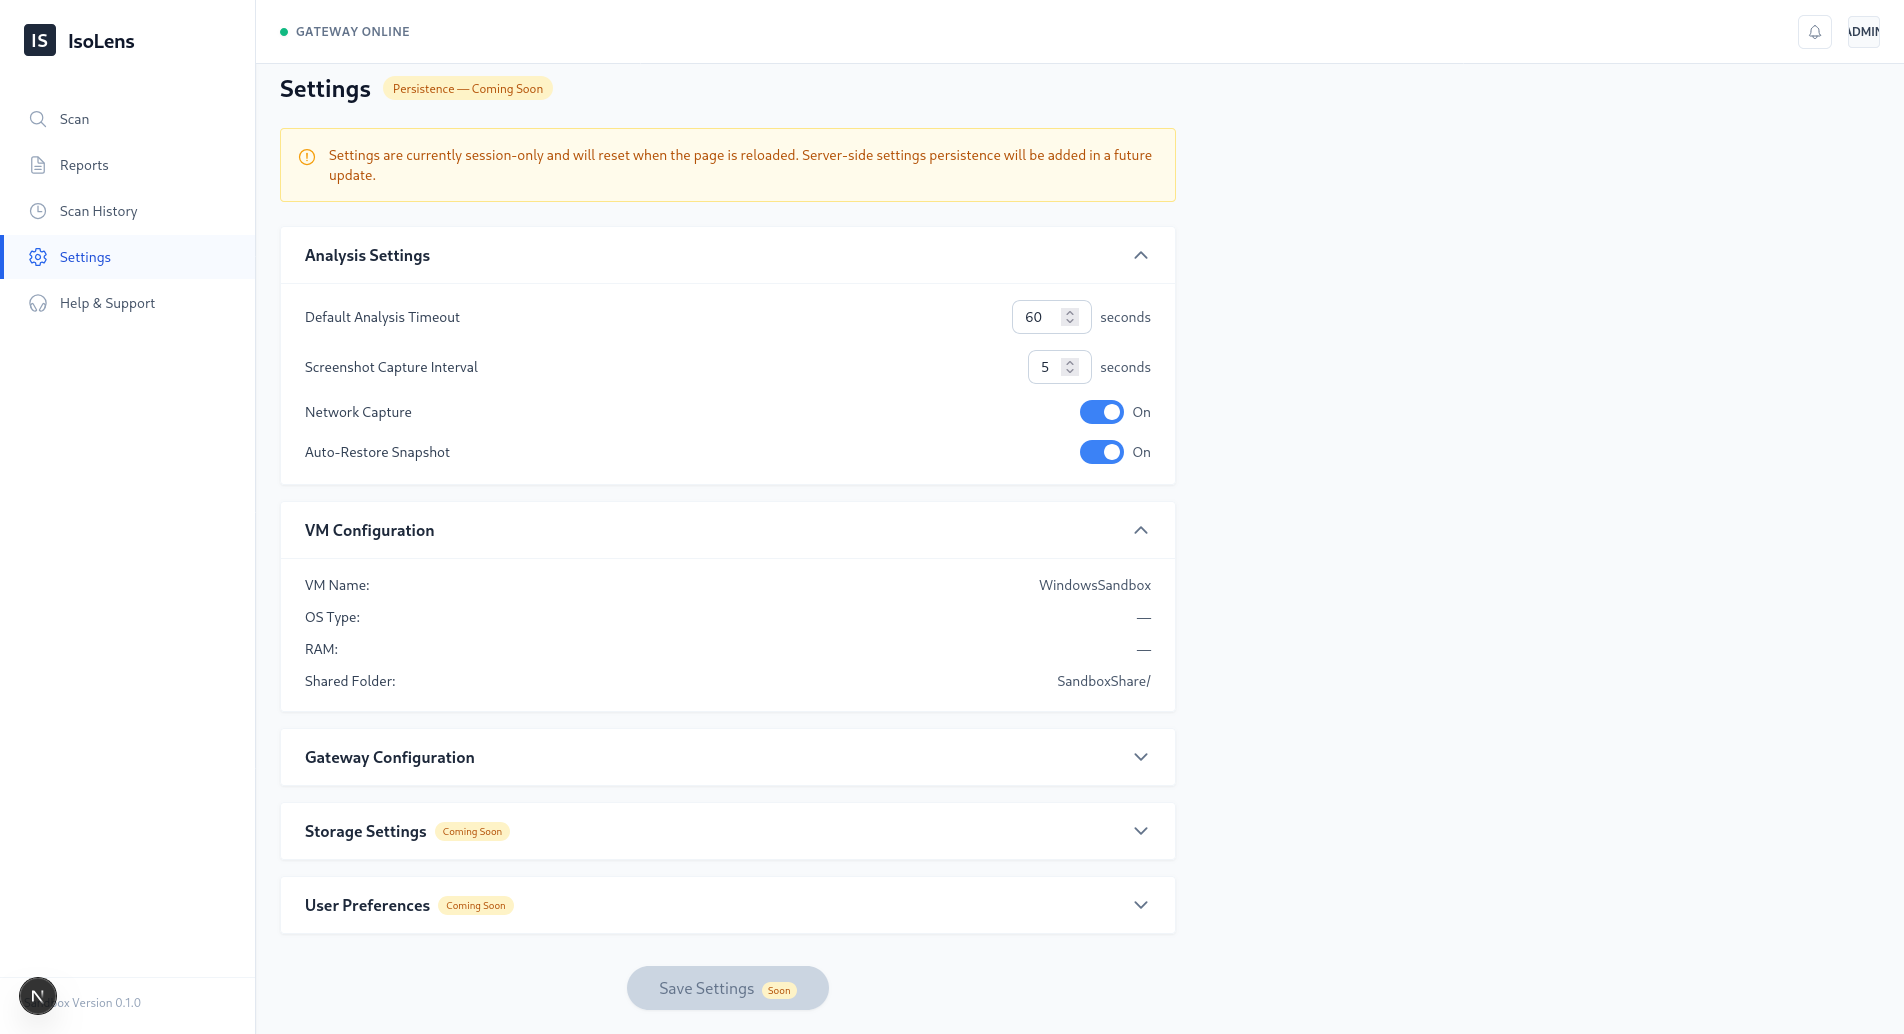
\includegraphics[width=0.92\textwidth]{figure/ui_settings_new.png}
\caption{Settings page for configuring sandbox and analysis preferences.}
\label{fig:settings_page}
\end{figure}
\begin{figure}[H]
\centering
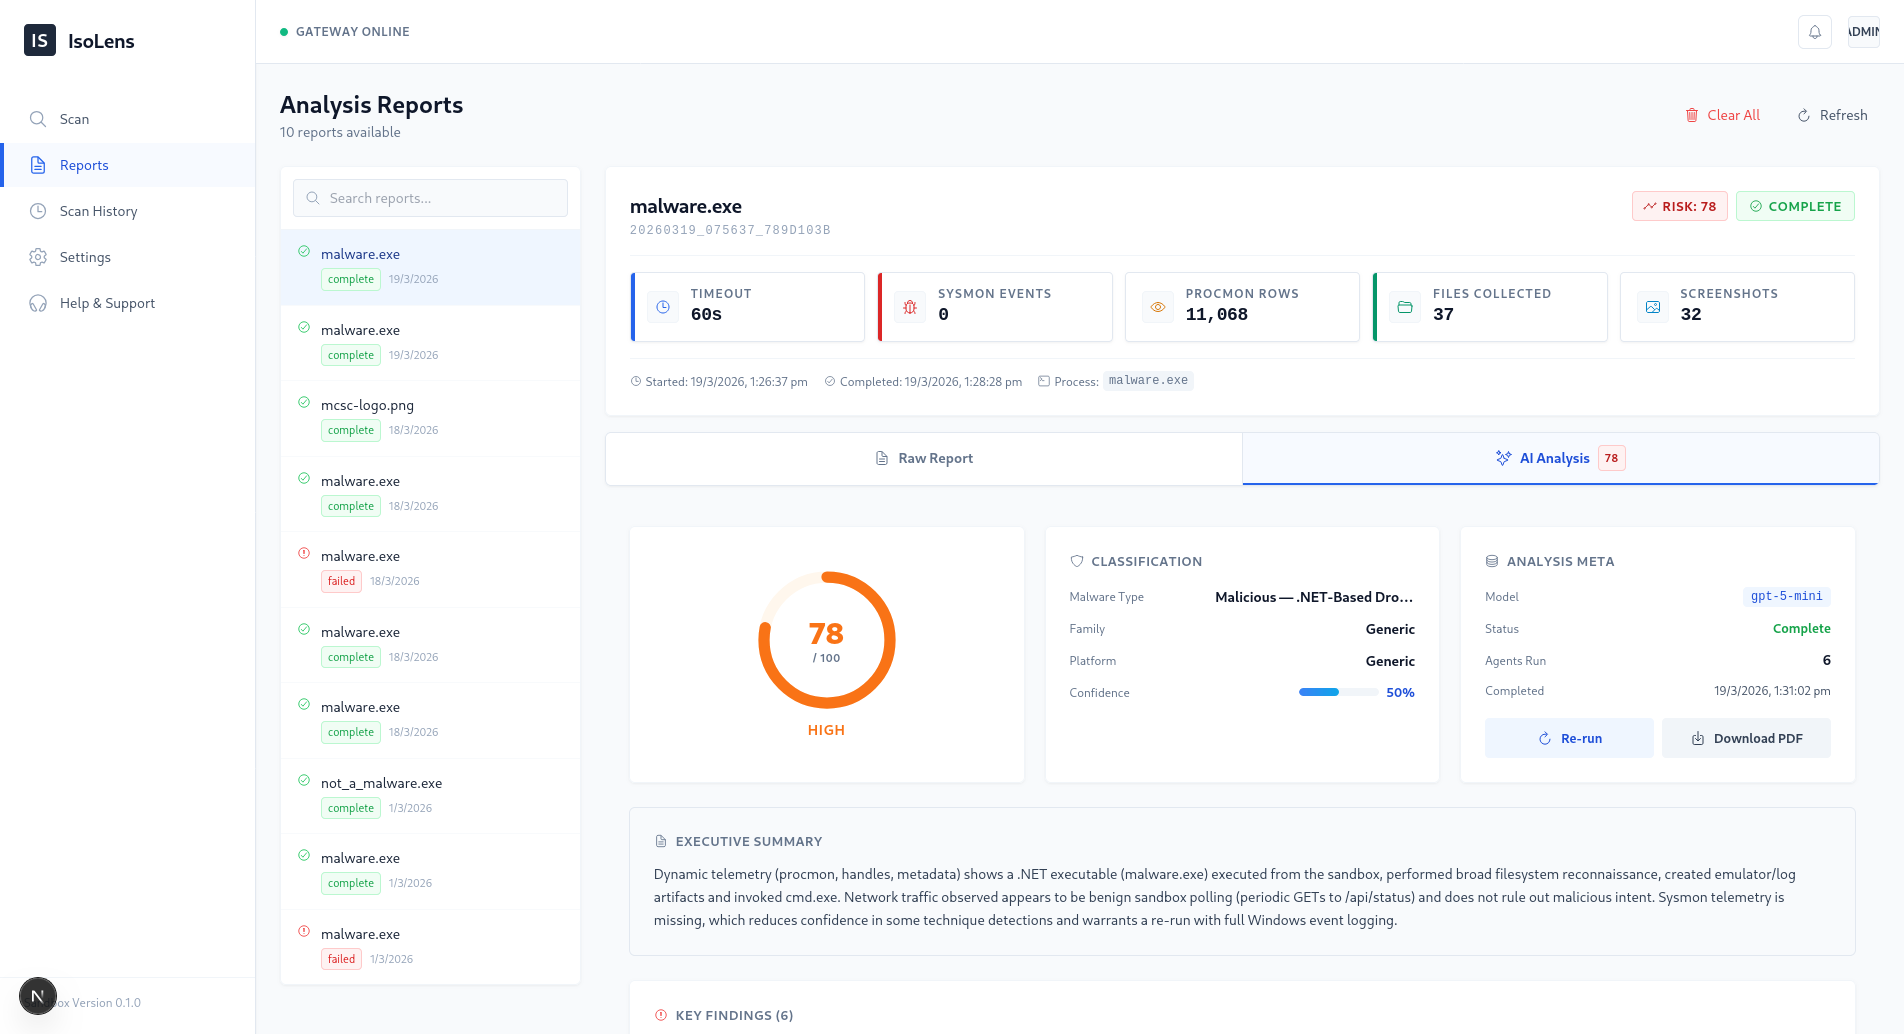
\includegraphics[width=0.92\textwidth]{figure/ui_ai_summary.png}
\caption{AI summary view showing consolidated intelligence findings and report output.}
\label{fig:ai_summary}
\end{figure}

\end{document}
